\documentclass[10pt]{beamer}

% Theme Selection
\usetheme{Madrid}
\usecolortheme{default}

\usepackage[style=apa,backend=biber]{biblatex}
\addbibresource{refs.bib}

\usepackage{tikz}
\usepackage{tikz-cd}
\usetikzlibrary{positioning, arrows.meta, shapes, calc, fit}
\usepackage{graphicx}
\usepackage{amsthm}

% Metadata
\title{Mycelial Brain}
\author{Luis Luarte}
\date{\today}

\begin{document}
	

	\begin{frame}
		\titlepage
	\end{frame}
	
	\begin{frame}
		\frametitle{The Mycelial intuition}
		\begin{itemize}
			\item \textbf{The problem:} financial market present highly non-stationary structure, often destroying trading strategies during regime shifts
			\item \textbf{The natural solution:} biological organisms thrive in ecosystems with regimes shifts in resources; often using simple local rules that provide an apparent solution to complex non-stationary structures
			\item \textbf{Uncertainty:} organisms often use "metabolic stress" (failure to find nutrients) as a proxy for environmental uncertainty, triggering a shift in their search strategy from exploitation to exploration
			\item \textbf{Mycelial networks:} present a exemplar case of solving the exploration/exploitation dilemma using extremely simple physical mechanisms
		\end{itemize}
		On a personal note I find mycelium fascinating, and I wanted to abstract its mechanisms for solving ecological problem into more abstract problems of higher-frequency trading
	\end{frame}
	
	\begin{frame}
		\frametitle{The mycelial mechanism}
		\begin{figure}
		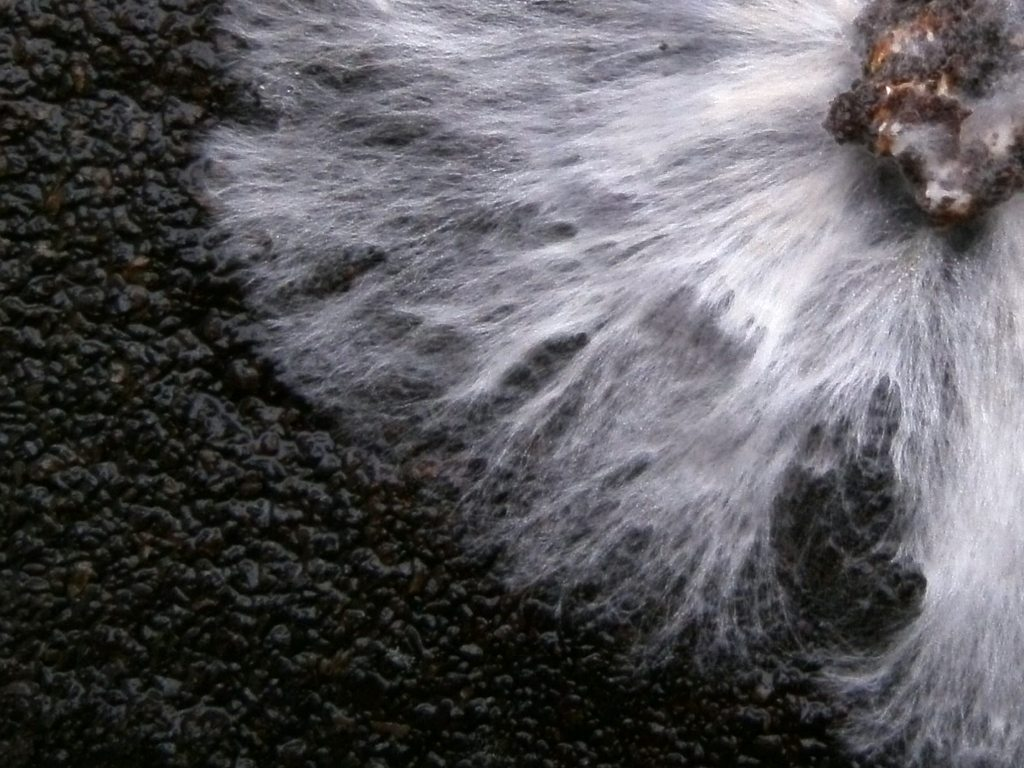
\includegraphics[width=0.5\textwidth]{mycelium.jpg}
		\caption{Mycelium is the main vegetative part of the organism, consisting of a vast, interconnected network of thread-like filament called hyphae. Typically grows submerged within a substrate and functions as the primary growing and feeding structure responsible for colonizing environment. Importantly it does not have a brain}
		\end{figure}
	\end{frame}
	
	\begin{frame}
		\frametitle{The vesicle supply center}
		\begin{equation}
			dV(\phi) = \frac{\dot{N} \cdot \cos(\phi)}{4\pi \cdot r^2}
			\end{equation}
			where:
			\begin{itemize}
				\item $dV(\phi)$ is the rate of wall surface expansion at angle $\phi$
				\item $\dot{N}$ the total rate of vesicle supply from the vesicle supply center
				\item $r$ is the distance from the VSC to the specific point on the cell
				\item $\phi$ is the angle between the point on the wall and the direction of growth
			\end{itemize}
			Then:
			\begin{equation}
				x_{VSC}(t + \Delta t) = x_{VSC}(t) + (v_{arrival} - v_{fusion}) \Delta t
			\end{equation}
			if:
			\begin{itemize}
				\item $v_{arrival} > v_{fusion}$ brownian motion
				\item $v_{arrival} < v_{fusion}$ diffusive motion
			\end{itemize}
	\end{frame}
	
	\begin{frame}
		\frametitle{Exploration vs. Exploitation}
		As resources become sparse (high risk/low reward), the optimal search strategy must shift from Brownian to Lévy (ballistic) to avoid over-sampling depleted zones \parencite{viswanathanOptimizingSuccessRandom1999}
		
		So my though process was
		\begin{itemize}
			\item Instead of a tedious process of mapping all vesicle mechanics lets focus on how their movement distributions change with nutrient supply
			\item The probability of taking $P(L) \sim L^{-(\mu)}$
			\item and then I needed $F: \text{Nutrient} \rightarrow \mu$
			\item so I defined: $\mu_{base} = \mu_{base} + \alpha \cdot tanh(\gamma \cdot \Delta_{\phi}(t))$
		\end{itemize}
		where:
		\begin{itemize}
			\item $\Delta \phi(t) = \phi_{arrival} - \phi_{fusion}(t)$
			\item $\phi_{\text{arrival}}(t) = R(t) + e^{-\lambda} \cdot \phi_{\text{arrival}}(t-1)$
			\item $\phi_{fusion}(t) = \phi_{arrival}(t) \cdot (1 - \sigma_{t})$
		\end{itemize}
	\end{frame}
	
		\begin{frame}
			\frametitle{Intuition}
			The intuition is to abstract the mechanism by modulating the movement distribution and letting the modulators be financial market variables, such as returns $\phi_{arrival}$ and risk $\phi_{fusion}$, while preserving the biological properties increased resources/returns increases Brownian movement, and adverse conditions high salinity/risk inhibit fusion increasing diffusivity.
		\end{frame}
		
		\begin{frame}
			\frametitle{Link with financial markets}
			How can I make mycelium navigate markets?
			My answer was to build a very simple topology
			\begin{itemize}
				\item The search topology is the set of all possible price coordinates (lags) the agent considers ``reachable'' at time $t$
				\item The agent is embedded because the search rules $(\mu)$ are defined in the same units and dimensions as the market's price lags
				\item The challenge then was if the agent is embedded with a logic that deals with regime changes can it survive the SP500 volatility?
			\end{itemize}
		\end{frame}
		
		\begin{frame}
			\frametitle{Financial market formalization}
			\begin{itemize}
				\item The market is a $d$-dimensional (2 for now) surface $\mathcal{M}$ where each point $x \in \mathcal{M}$ represents a state in the \textbf{lag-phase space}
				\item Coordinates: a point $x_{t} = (P_{t-1}, P_{t-2},\dots, P_{t-d})$ where $P$ are the $log$ price return of SP500 1927-2020
				\item The agent moves to a coordinate $x$ using a Levy distribution with $\mu$ exponent
				\item It generate the hypothesis that the market pattern is best explained by this two price lags (1, 2) a fast and a slow structure
				\item It scans a past return window of size $n$ computing the euclidean distance between (1, 2) and every other pair ($L_{1}, L_{2}$) using returns and those lags
				\item When it finds a close neighbor it look at what happened next and uses that as a prediction
			\end{itemize}
		\end{frame}
		
		\begin{frame}
			\frametitle{The final loop}
			\begin{itemize}
			\item The prediction is $\hat{y}_t = \frac{\sum_{\tau=t-W}^{t-1} R_{\tau+1} \cdot K_{\mu}(\| \mathbf{x}_t - \mathbf{x}_{\tau} \|)}{\sum_{\tau=t-W}^{t-1} K_{\mu}(\| \mathbf{x}_t - \mathbf{x}_{\tau} \|)}$
			\item with Kernel $K_{\mu}(d) = \exp\left( -\frac{d^2}{2\ell(\mu)^2} \right)$
		\end{itemize}
		The intuition is that $\| \mathbf{x}_t - \mathbf{x}_{\tau} \|$ represent how close the current market feels to a past pattern, and the kernel allows $\mu$ to weight this ``distance''
		Then the reward is defined by $R_t = \text{sgn}(\hat{y}_t \cdot y_{t+1}) \cdot \ln\left( 1 + |y_{t+1}| \right) - \Omega(\sigma_t)$
		Where
		\begin{itemize}
			\item $\text{sgn}(\hat{y}_t \cdot y_{t+1})$ is the directional alignment of real and predicted returns
			\item $\ln\left( 1 + |y_{t+1}| \right)$ is the nutrient density with log to simulate diminishing returns of energy intake, agent eats the return magnitude
			\item $\Omega(\sigma_t)$ is the metabolic cost of existing in a volatile $\sigma$ environment, this represent the high salinity of the environment
			\item $\phi_{\text{arrival}}(t) = \max(0, R_t) + e^{-\lambda} \cdot \phi_{\text{arrival}}(t-1)$
			\item Agent position rewards determines its future movement, many steps to a simple idea
		\end{itemize}
		\end{frame}
		
		\begin{frame}
			\frametitle{Deriving market risk}
			Finally the agent derives market risk as:
			\begin{equation}
				\sigma_t = \text{Clip} \left( \frac{\text{Std}(R_{t-W:t}) \cdot \sqrt{\text{MA}(|y - \hat{y}|_{t-W:t})}}{\sigma_{\text{baseline}}} \right)
			\end{equation}
			Where
			\begin{itemize}
				\item $Std(R_{t-W:t})$ is the standard deviation of the returns in the window, represent mechanical stress of the market substrate
				\item $MA(\left|y-\hat{y}\right|_{t-W:t})$ the moving average of the absolute prediction error
				\item $\sigma_{baseline}$ long term volatility to keep everything in a reasonable range
			\end{itemize}
		\end{frame}
		
		\begin{frame}
			\frametitle{Testing the agent}
					\begin{figure}
				\includegraphics[width=0.70\textwidth]{p1.pdf}
				\caption{The substrate consists of SP 500 daily log-returns 1927-2020. We employed a bootstrap-sampling method with a rolling 100-day history window to generate 1000 discrete "ticks". For each tick, the agent’s internal Risk Metric was derived from a composite of realized volatility and topological prediction error, while the Lévy Exponent was modulated by flux imbalance controller}
			\end{figure}
			\begin{itemize}
				\item \textbf{Bifurcation of search:} agents produces distinct clusters that change over time and are modulated by the risk metric, $\mu$ strategy seems to change with regime changes
				\item \textbf{The "gap":} the sparse region in the center suggest a zone where the agent rarely lingers, preferring rapid phase transitions to preserve metabolic integrity
			\end{itemize}
		\end{frame}
		
		\begin{frame}
			\frametitle{Testing the agent}
			\begin{figure}
				\includegraphics[width=0.70\textwidth]{p2.pdf}
				\caption{Hartigans's Dip test rejects unimodality of $\mu$ exponent with $D = 0.0012$ and $p<0.01$}
			\end{figure}
		\end{frame}
		
		
				\begin{frame}
			\frametitle{Testing the agent}
			\begin{figure}
				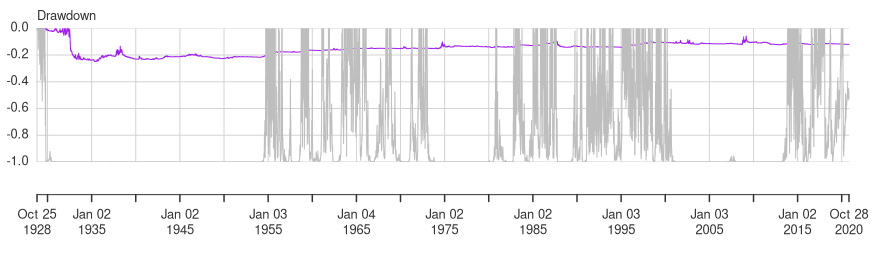
\includegraphics[width=0.70\textwidth]{p3.png}
				\caption{$DD_T = \frac{W_T - \max_{t \in [0, T]} (W_t)}{\max_{t \in [0, T]} (W_t)}$, peak-to-trough decline during a specific period for a trading acount, critical metric for higher frequency trading, the agent ``learn'' to hibernate when volatility is high}
			\end{figure}
			\end{frame}
			
		\begin{frame}
				\frametitle{Testing the agent}
				\begin{figure}
					\includegraphics[width=0.70\textwidth]{p4.pdf}
					\caption{Two topological phases emerge with fast transitions}
				\end{figure}
		\end{frame}
		
		\begin{frame}
			\frametitle{Discussion}
			\begin{itemize}
				\item Proof of concept of how simple nature-based rule can deal with volatile market regime changes
				\item Agent phase transitions between exploitation and exploration with good timing preventing large drawdowns
				\item future work: can we generate a trading strategy with this?
				\item how to implement chemical signaling between agents
				\item can we capture fungal ``species'' algorithms, how could we parametrize or abstract that?
			\end{itemize}
		\end{frame}

	
	
	
\end{document}